\begin{frame}{Fundamentação Teórica}{Análise de Funcionamento e Aplicação de Uma cisterna}

\vspace{-1}
\begin{itemize}
\justify{\small{Para desenvolvimento do trabalho, parte-se do princípio de uma estrutura previamente construída, demostrada na figura.} }
\end{itemize}


\vspace{-0.64}
\begin{figure}[htp]
	\centering
	\caption{\small{Esquema de demonstração de uma cisterna no subsolo.}}
	\label{figura01}
	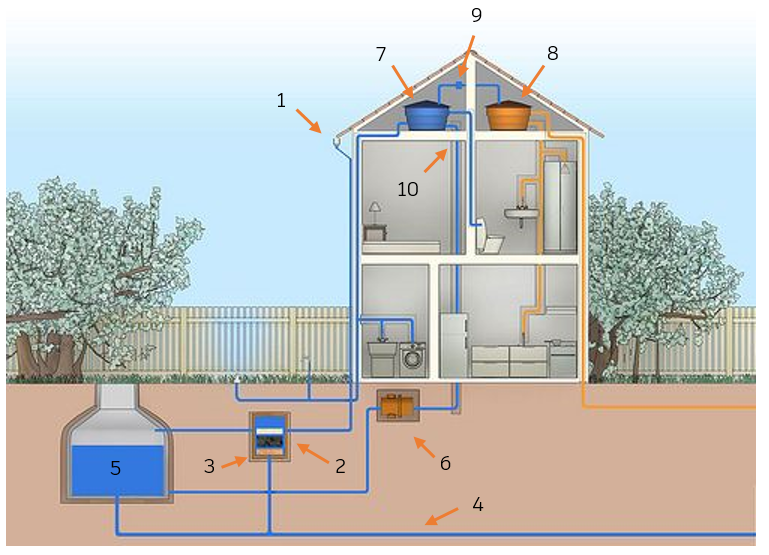
\includegraphics[width=0.5\linewidth]{figuras/esquema_cisterna.png}
   % \vspace{3cm}
    \hspace{5cm}
	\legend{\small{Fonte: Adaptado (ECOMONTES, 2016)}}
\end{figure}
    
\end{frame}

\begin{frame}
\resizebox{10cm}{!}{
\begin{table}[]
	\centering
	\small
	\begin{tabular}{c|c|c}
		\hline
		\textbf{Identificador} & \textbf{Elemento} & \textbf{Descrição} \\ \hline
		1 & Calha coletora & \begin{tabular}[c]{@{}c@{}}Elemento convencional para coleta e \\ descarte de água da chuva\end{tabular} \\ \hline
		2 & Filtro A (cascalho fino) & \begin{tabular}[c]{@{}c@{}}Elemento para realização de \\ filtragem de pequenas impurezas\end{tabular} \\ \hline
		3 & Filtro B (cascalho grosso) & \begin{tabular}[c]{@{}c@{}}Elemento para realização de \\ filtragem de impurezas\end{tabular} \\ \hline
		4 & Tubulação de descarte & \begin{tabular}[c]{@{}c@{}}Tubulação utilizada como rota de escoamento \\ quando o reservatório não está em uso ou \\ está cheio\end{tabular} \\ \hline
		5 & Reservatório de coleta & Cisterna propriamente dita \\ \hline
		6 & Motobomba ou bomda d'água & \begin{tabular}[c]{@{}c@{}}Elemento utilizado para realização do \\ ganho de elevação da água\end{tabular} \\ \hline
		7 & Caixa d'água auxiliar & \begin{tabular}[c]{@{}c@{}}Caixa d'água convencional com alimentação \\ oriunda da bomba d'água\end{tabular} \\ \hline
		8 & Caixa d'água convencional & \begin{tabular}[c]{@{}c@{}}Caixa d'água padrão com alimentação \\ da estação de água da cidade\end{tabular} \\ \hline
		9 & Elo de ligação & \begin{tabular}[c]{@{}c@{}}Ligação utilizada para abastecer a caixa d'água \\ auxiliar quando a cisterna está seca \\ ou em manutenção\end{tabular} \\ \hline
		10 & Distribuidor & \begin{tabular}[c]{@{}c@{}}Elementos de distribuição de água \\ para pontos estratégicos\end{tabular} \\ \hline
	\end{tabular}
	\caption{Identificação dos elementos da \autoref{fig:esquema_cisterna}.}
	\label{tab:tabela_esquema_cisterna}
\end{table}
}

\end{frame}

\begin{frame}{Fundamentação Teórica}{O \textit{Framework} SmartLVGrid}
\begin{itemize}

\end{itemize}
\begin{block}{SmartLVGrid}
\justify{\textit{Framework} que realiza a convergência de sistemas legados de baixa tensão em sistemas inteligentes, utilizando a estratégia do \textit{retrofit}. Ele possui como elemento básico de funcionamento a Unidade de Comunicação e Automação, ACU, sendo classificada em \textit{operator}, \textit{sub-coordinator} ou \textit{coordinator}.}
\end{block}    
\medskip
\justify{Este \textit{framework} possibilita:
\begin{enumerate}
\item transição tecnológica de baixo custo;
\item adição de elementos de controle e monitoramento aos sistemas elétricos de baixa tensão;
\item mantimento das infraestruturas já existentes.}
    \end{enumerate}
\end{frame}

\begin{frame}{Fundamentação Teórica}{SmartLVGrid}
\vspace{-0.64cm}
\begin{figure}[htp]
	\centering
	\caption{\centering{\small{Pilha SmartLVGrid}}}
	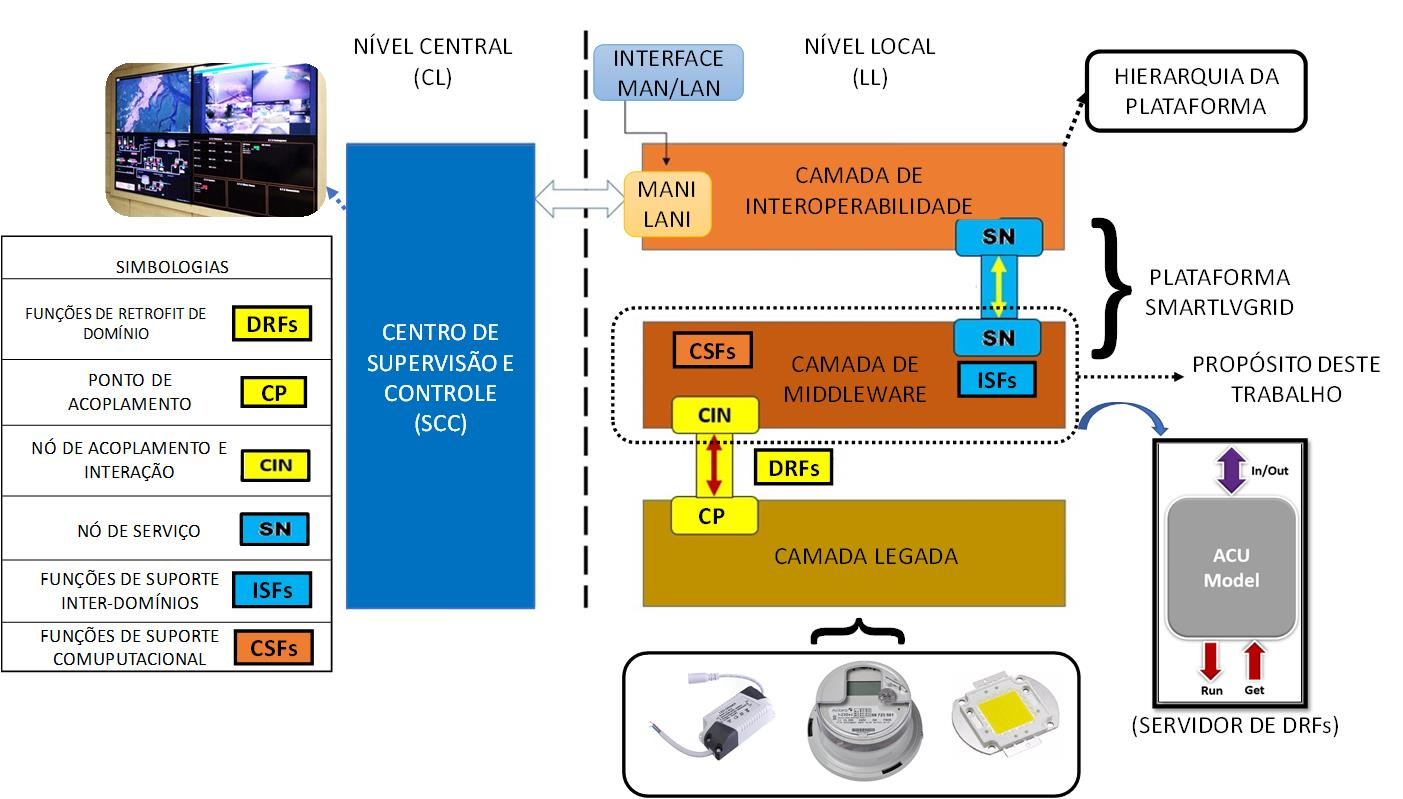
\includegraphics[width=0.95\linewidth]{img/PILHASLVG.jpg}
        \hspace{5cm}
    \vspace{5cm}
	\legend{\small{Fonte: Adaptado \cite{gomes,fernandes2018implementation,medidor,gomes2019smartlvgrid}}}
\end{figure}
\end{frame} 

\begin{frame}{Fundamentação Teórica}{O ACU}
\vspace{-0.64cm}
\begin{figure}[htp]
	\centering
	\caption{\centering{\small{Composição de um elemento ACU}}}
	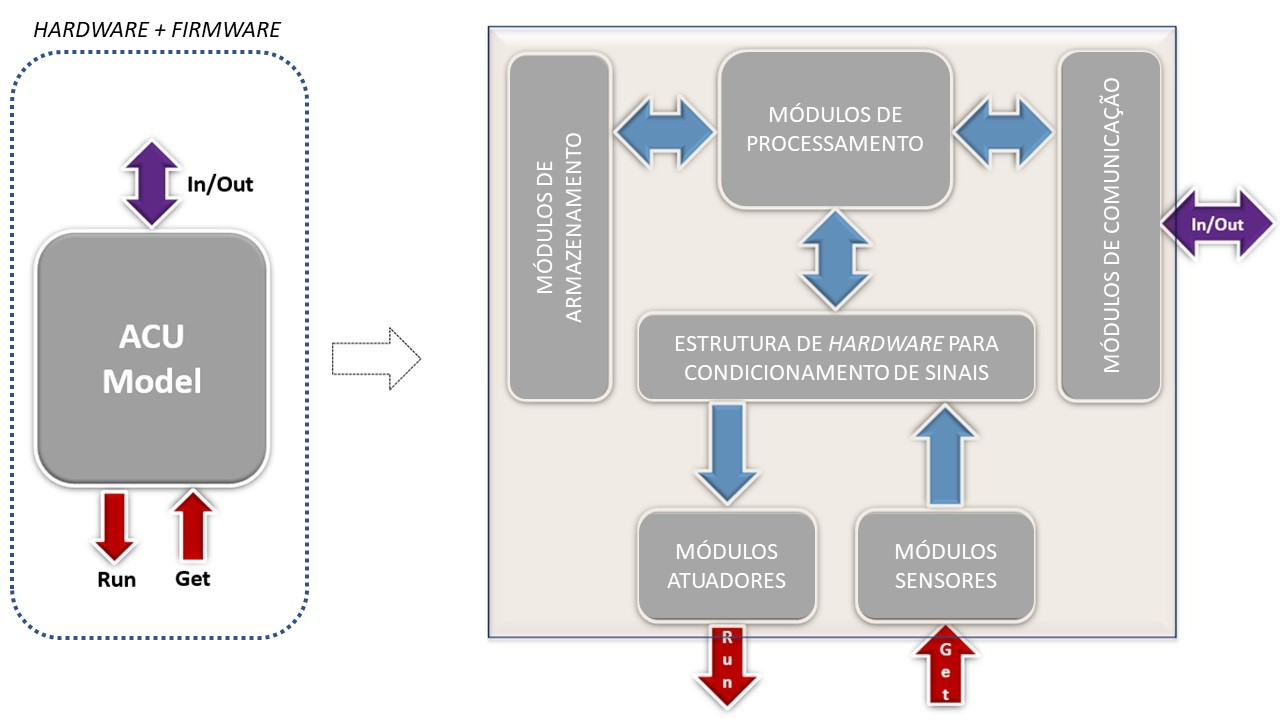
\includegraphics[width=0.97\linewidth]{img/ACU.jpg}
    \hspace{5cm}
        \vspace{5cm}
	\legend{\small{Fonte: Adaptado \cite{gomes,gomes2019smartlvgrid}}}
\end{figure}
\end{frame}

\begin{frame}{Fundamentação Teórica}{Controle Eficiente para Sistemas de Iluminação LED}
\vspace{-0.64cm}
\begin{figure}[htp]
	\centering
	\caption{\centering{\small{Sistema de controle PFC}}}
	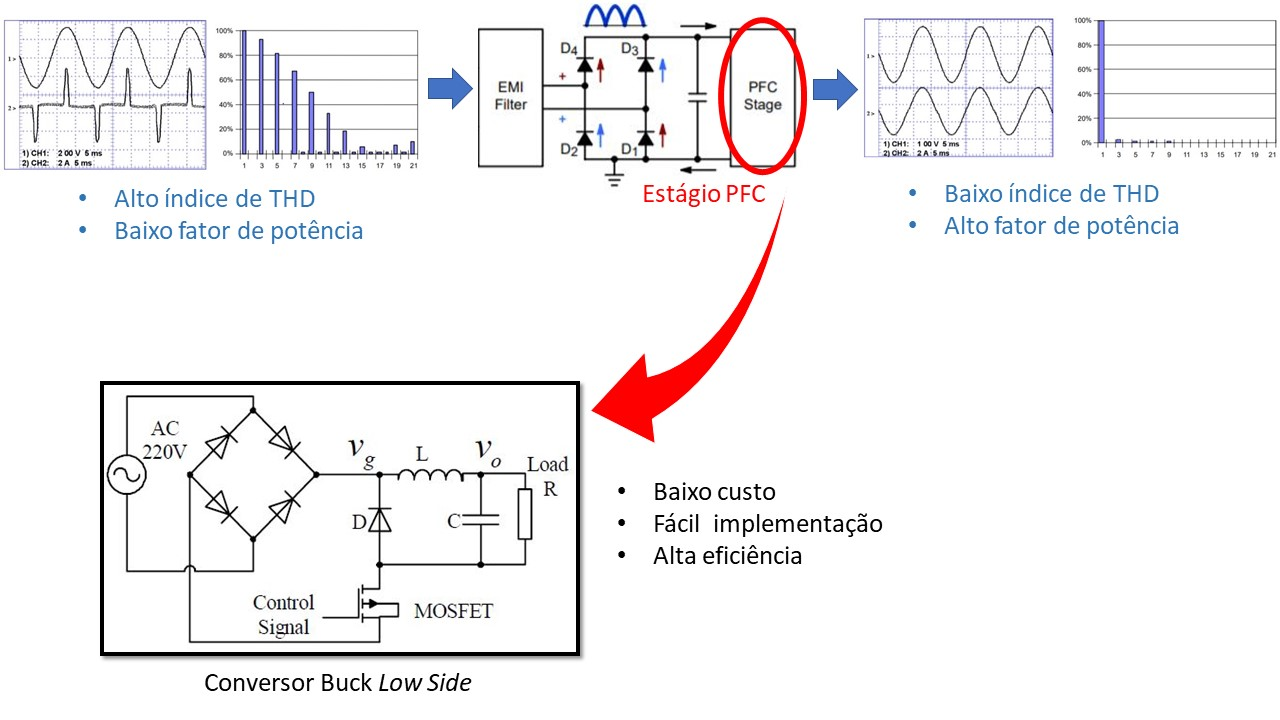
\includegraphics[width=0.97\linewidth]{img/pfc_.jpg}
    \hspace{5cm}
    \vspace{5cm}
	\legend{\small{Fonte: Adaptado \cite{semiconductor2007power,xiangrong2006low}}}
\end{figure}
\end{frame}

\begin{frame}{Fundamentação Teórica}{Sistemas Inteligentes para Medição dos Parâmetros Elétricos}
\vspace{-0.64cm}
\begin{figure}[htp]
	\centering
	\caption{\centering{\small{Composição de um \textit{smart meter}}}}
	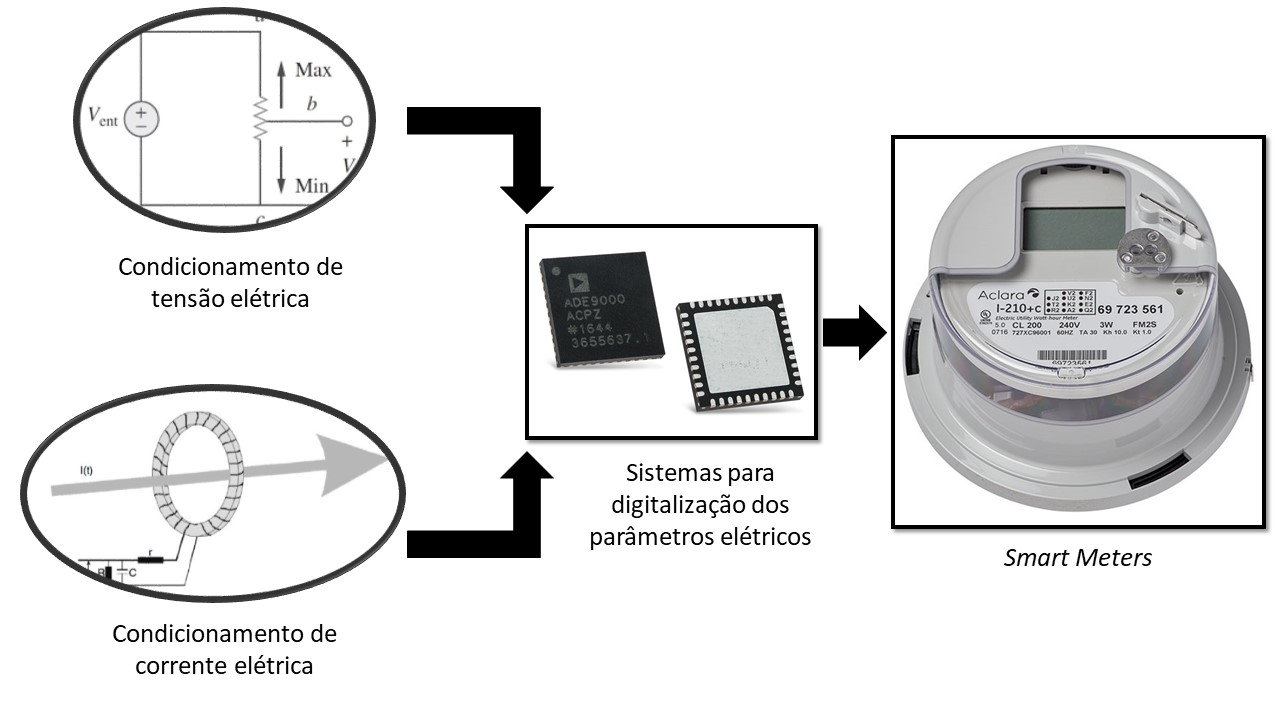
\includegraphics[width=0.97\linewidth]{img/smeter.jpg}
    \hspace{5cm}
    \vspace{5cm}
	\legend{\small{Fonte: Adaptado \cite{alexander2013fundamentos,samimi2013review,medidor,ADE9000}}}
\end{figure}
\end{frame}

\begin{frame}{Fundamentação Teórica}{Chaves Estáticas de Transferência de Energia}
\vspace{-0.64cm}
\begin{figure}[htp]
	\centering
	\caption{\centering{\small{Chave de transferência estática aplicado a uma carga monofásica}}}
	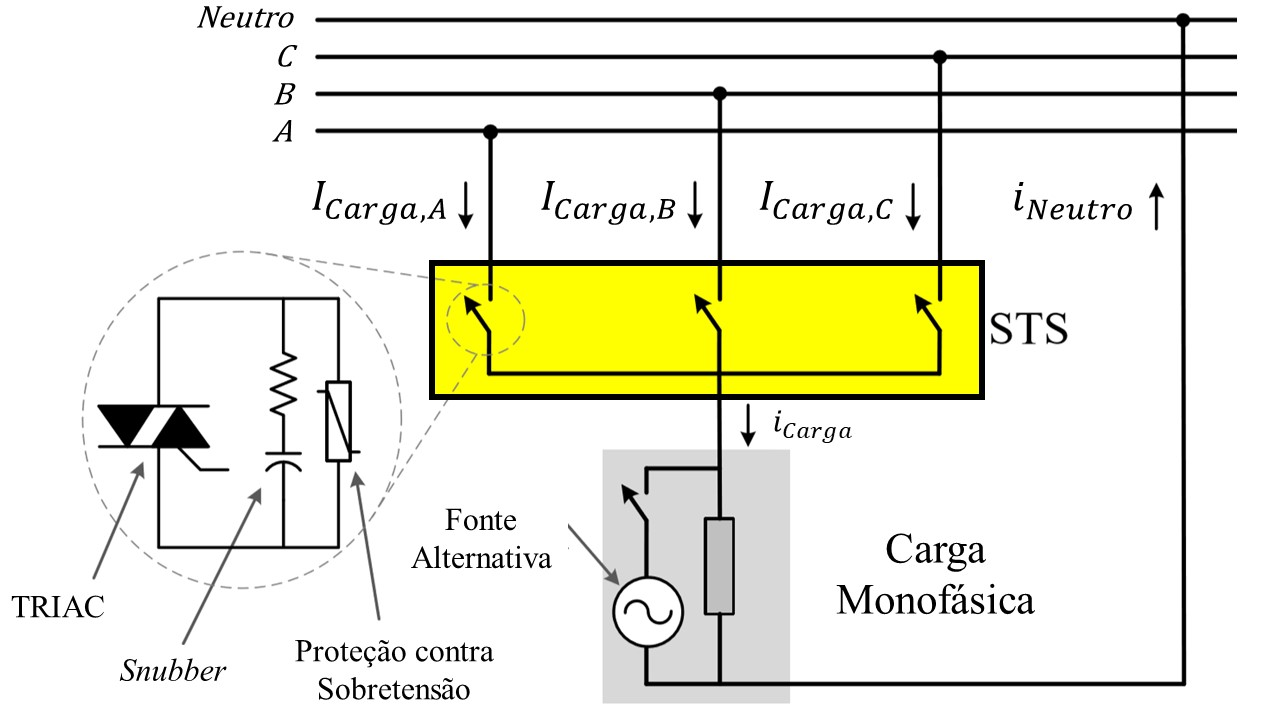
\includegraphics[width=0.97\linewidth]{img/STS.jpg}
    \hspace{5cm}
	\legend{\small{Fonte: Adaptado \cite{shahnia2014voltage}}}
\end{figure}
\end{frame}























